\documentclass[12pt, a4paper, portrait]{article}
%Gummi|065|=)
\usepackage[affil-it]{authblk}
\usepackage{hyperref}
\hypersetup{
  colorlinks=true,
  linkcolor=black,
  filecolor=magenta,
  urlcolor=blue
}
\urlstyle{same}
\usepackage{indentfirst}
\usepackage{courier}
\usepackage{listings}
\usepackage{color}
\definecolor{codegreen}{rgb}{0,0.6,0}
\definecolor{codegray}{rgb}{0.5,0.5,0.5}
\definecolor{codepurple}{rgb}{0.58,0,0.82}
\definecolor{backcolour}{rgb}{0.95,0.95,0.92}
\lstdefinestyle{mystyle}{
    backgroundcolor=\color{backcolour},   
    commentstyle=\color{codegreen},
    keywordstyle=\color{magenta},
    numberstyle=\tiny\color{codegray},
    stringstyle=\color{codepurple},
    basicstyle=\ttfamily\footnotesize,
    breakatwhitespace=false,         
    breaklines=true,                 
    captionpos=b,                    
    keepspaces=true,                 
    numbers=left,                    
    numbersep=5pt,                  
    showspaces=false,                
    showstringspaces=false,
    showtabs=false,                  
    tabsize=2
}
 
\lstset{style=mystyle}

\usepackage{indentfirst}
\usepackage[utf8]{inputenc}

\usepackage{geometry}
\geometry{
 a4paper,
 left=20mm,
 top=20mm,
 right=25mm,
 bottom=20mm
}

% Personal data
\title{\textbf{Sensor Music Player}}
\author{István Szőllősi}
\affil{Faculty of Sciences and Letters, ``Petru Maior'' University of Târgu Mureș}
\date{August 25, 2018}

\renewcommand{\baselinestretch}{1.5} 
\usepackage{graphicx}
\begin{document}

\maketitle
\newpage

\tableofcontents
\newpage

\section{About}
The project is committed to the GitHub, you can find \href{https://github.com/I-sty/SensorMusicPlayer/}{here}.
\par The main structure of the repository is
\textit{a valid Android project} with several additionals folders, like the:
\begin{itemize}
\item{\textbf{backend}} folder where the \textit{Python} and \textit{JavaScript} codes are stored
\item{\textbf{docs}} folder where the documents about the project are stored
\end{itemize}

\pagebreak
\section{Node.js}
In Node.js is very simple to create a small web server for REST calls.
\subsection{Installation}
\subsection{Usage}
To start use the follow command in the project's folder:
\begin{lstlisting}[language=bash]
npm run start
\end{lstlisting}
\subsection{Configuration}
Used tutorial: \href{https://www.codementor.io/olatundegaruba/nodejs-restful-apis-in-10-minutes-q0sgsfhbd}{Build Node.js RESTful APIs in 10 Minutes}
\subsubsection{Mongoose}
\subsubsection{Express}
\subsubsection{Nodemon}

\pagebreak
\section{MongoDB}
MongoDB to store signal data from the \textit{Y axis} of the accelerometer from the Android devices.
\subsection{Installation}
\subsection{Runing}
To start mongo service use the follow command:
\begin{lstlisting}[language=bash]
sudo mongod --config /etc/mongodb.conf 
\end{lstlisting}
To access the mongo shell enter the \textit{mongod} command in terminal.
\subsection{Drop collection}
Code:
\begin{lstlisting}[language=bash, caption=MongoDB shell commands to drop a collection]
show dbs
use <db>
show collections
db.<collection>.drop()
\end{lstlisting}

\pagebreak
\section{Matplotlib}
Matplotlib is a plotting library for the Python programming language.
I used \textit{matplotlib} to generate graphical view of my series.
\subsection{Installation}
Install module using this \href{https://matplotlib.org/users/installing.html#linux-using-your-package-manager}{tutorial}.
\par Optionally, you need to install the \textbf{python-tk} package also.
\subsection{Examples}
According to this \href{https://matplotlib.org/users/pyplot_tutorial.html}{official tutorial} you can easily generate a plot about an array using this Python script:
\begin{lstlisting}[language=Python]
import matplotlib.pyplot as plt
plt.plot([ 5.733, 1.704, -2.713, -1.343, 2.604, 3.922, 2.157, -0.910, -2.414, -2.943, -1.526, -0.823])
plt.ylabel('some numbers')
plt.show()
\end{lstlisting}

Result:
\begin{figure}[ht]
\centering
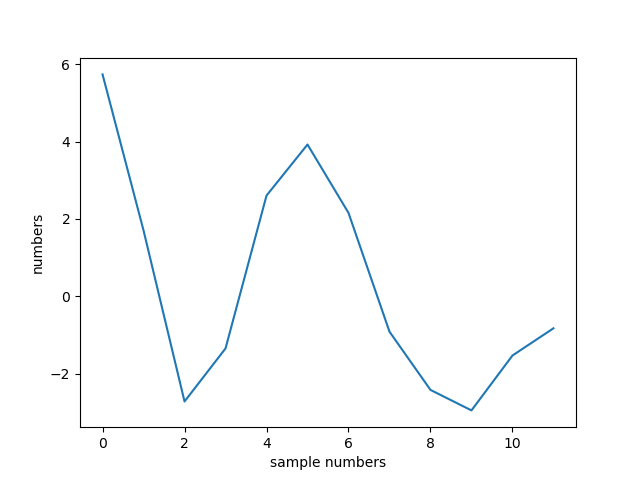
\includegraphics[scale=0.87]{Figure_2.png}
\caption{The result of the script}
\end{figure}
\clearpage
This example was very easy, so here is a \textit{normal} signal from the accelerometer:
\begin{figure}[htp]
\centering
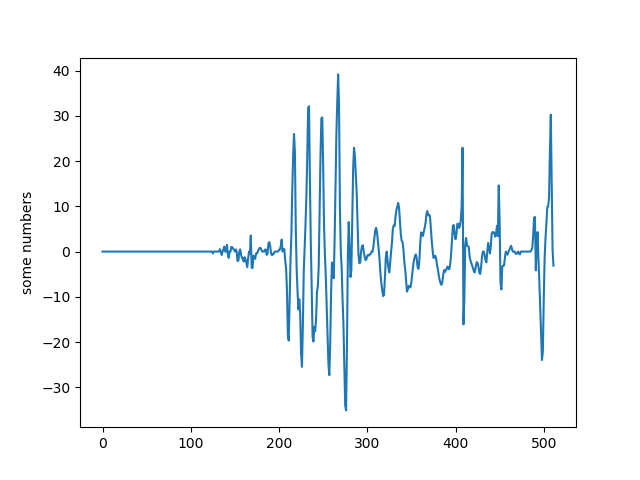
\includegraphics[scale=1.00]{Figure_1.png}
\caption{A section of the signal of accelerometer in real usage}
\end{figure}

\pagebreak
\section{DTAIDistance}
Library for time series distances (e.g. Dynamic Time Warping) used in the \href{https://dtai.cs.kuleuven.be/}{DTAI Research Group}.
\par
DTAIDistance official documentation: \href{https://dtaidistance.readthedocs.io/en/latest/index.html}{dtaidistance.readthedocs.io}
\par Source available on \url{https://github.com/wannesm/dtaidistance}.

\subsection{Installation}
Run the follow codes in terminal to install the module:
\begin{lstlisting}[language=bash, caption=Used Linux Mint 19]
sudo apt install python3-pip python3-setuptools  python3-dev python3-tk
pip3 install wheel
pip3 install dtw
pip3 install dtaidistance
\end{lstlisting}

\subsection{Usage}
\begin{lstlisting}[language=Python, caption=Script to calculate DTW distance and plot warping paths matrix ]
from dtaidistance import dtw
from dtaidistance import dtw_visualisation as dtwvis
import numpy as np

s1 = np.array([0, 1, 2, 1, 0, 2, 1, 0, 0])
s2 = np.array([0, 1, 2, 1, 0, 0, 1, 2, 1])

d, matrix = dtw.warping_paths(s1, s2, window=25, psi=2)
print('DTW distance = ', d)

dtwvis.plot_warpingpaths(s1, s2, matrix, best_path, "image.png")
\end{lstlisting}

\clearpage
The result will be put in the newly created \textbf{image.png} file.
\begin{figure}[ht]
\centering
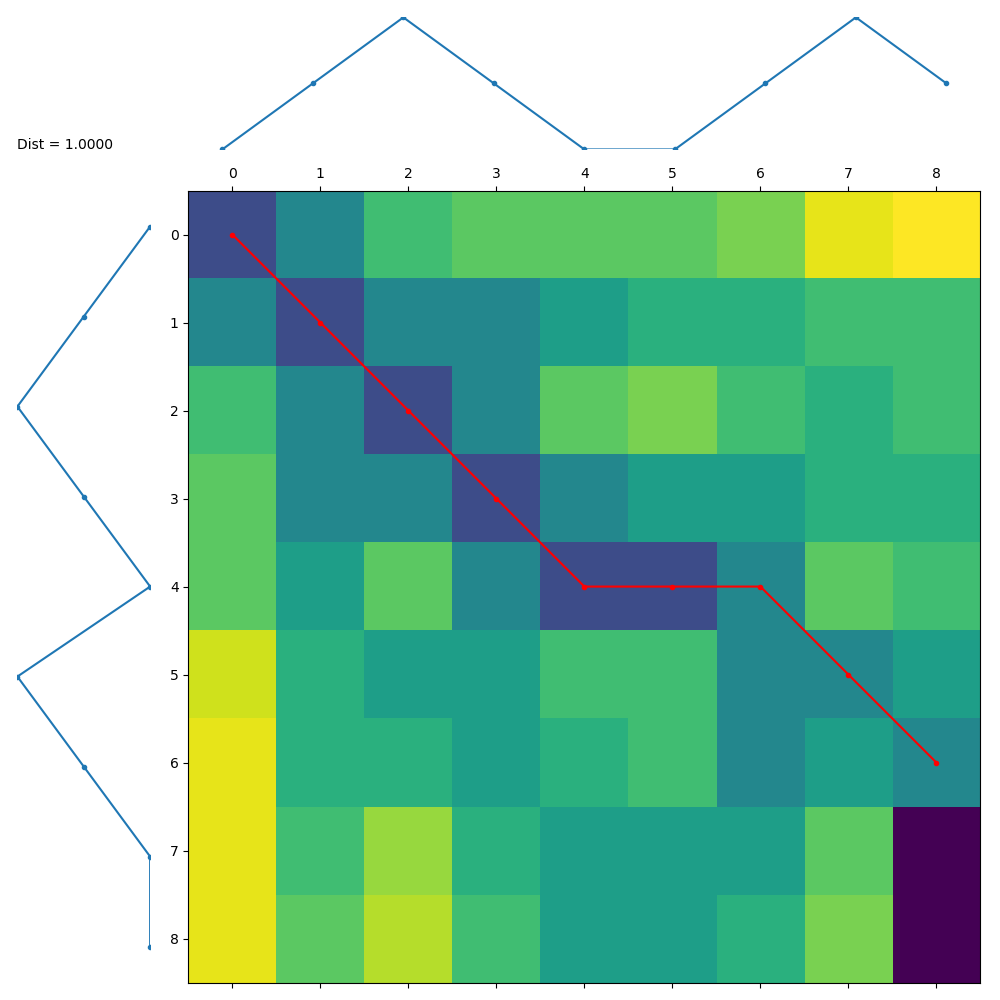
\includegraphics[scale=0.60]{dtaidistance-sample.png}
\caption{DTAIDistance's warping paths matrix}
\label{}
\end{figure}

\subsection{Documentation}
\begin{lstlisting}[language=Python]
import numpy as np
s1 = np.array([0, 1, 2, 1, 0, 2, 1, 0, 0])
\end{lstlisting}
\par\href{http://www.numpy.org/}{NumPy} is a library for the Python programming language, adding support for large, multi-dimensional arrays and matrices, along with a large collection of high-level mathematical functions to operate on these arrays.
\par The \textit{array()} function creates an array from a given list. See more details \href{https://docs.scipy.org/doc/numpy/reference/generated/numpy.array.html#numpy.array}{here}.
\newline
\begin{lstlisting}[language=Python]
from dtaidistance import dtw
d, matrix = dtw.warping_paths(s1, s2, window=25, psi=2)
print('DTW distance = ', d)
print('DTW matrix = ', matrix
\end{lstlisting}

\par The \textit{warping\_paths()} function calculates the DTW distance and the DTW matrix for the two given series. See more details
\href{https://dtaidistance.readthedocs.io/en/latest/modules/dtw.html?highlight=warping_paths#dtaidistance.dtw.warping_paths}{here}.
\newline

\begin{lstlisting}[language=Python]
from dtaidistance import dtw_visualisation as dtwvis
dtwvis.plot_warpingpaths(s1, s2, matrix, best_path, "image.png")
\end{lstlisting}
\par The \textit{plot\_warpingpaths()} method plots the warping paths matrix into the \textit{image.png} file. See more details \href{https://dtaidistance.readthedocs.io/en/latest/modules/dtw_visualisation.html}{here}.


\pagebreak
\section{Postman}
\subsection{Installation}
Installed according to this article: \href{https://r00t4bl3.com/post/how-to-install-postman-native-app-in-linux-mint-18-3-sylvia}{How to install Postman native app in Linux Mint 18.3}

Used to test the main functionalities of the Node.js server.

\subsection{Usage}
\subsubsection{GET}
To get all buffers from database run this code in Postman/Linux terminal
\begin{lstlisting}[language=bash, caption=Get all buffers]
curl -X GET http://localhost:3000/buffers
\end{lstlisting}

The response is or an empty list, if no items in the database or a list like this:
\begin{lstlisting}[language=XML, caption=A sub section of the signal to process]
[
    {
        "value": [
            5.733050346374512,
            1.704751968383789,
            -2.7134790420532227,
            -1.343064308166504,
            2.6042985916137695,
            3.92281436920166,
            2.15725040435791,
            -0.9106369018554688,
            -2.4146032333374023,
            -2.943338394165039,
            -1.5269522666931152,
            -0.8230304718017578
        ],
        "_id": "5b82607f5601ec575d3bf0e4",
        "__v": 0
    }
]
\end{lstlisting}

\subsubsection{POST}
Post a new buffer a.k.a a sub section of the signal to store and process. Run this code in Postman or in a Linux terminal to post a new buffer to the Node.js server.
\begin{lstlisting}[language=bash, caption=Send signal data via REST]
curl -X POST http://localhost:3000/buffers  -d '{
	"value":[-2.2, -1.1, 0, 1.1, 2.2]
}'
\end{lstlisting}

\pagebreak
\section{PyMongo}
\subsection{Installation}
\begin{lstlisting}[language=bash]
pip3 install pymongo
\end{lstlisting}
Installing with pip: \url{http://api.mongodb.com/python/current/installation.html}
\subsection{Usage}
\begin{lstlisting}[language=Python]
import pymongo
from pymongo import MongoClient
client = MongoClient('localhost', 27017)
client.database_names()
db = client['<db_name>']
db.collection_names()
coll = db['<collection_name>']

for col in coll.find({}):
    for keys in col.keys(): 
        print ('{', keys, ":" , col[keys] , '}' )
        
\end{lstlisting}

\end{document}
